%-----------------------------------------------------------------------------%
%                                                                             %
%    Anh�nge					                                             					  %
%                                                                             %
%-----------------------------------------------------------------------------%

\appendix
\chapter{Appendix}

\section{CoP Cost Implementation for Contact Dynamics}\label{app:ContactCoP}
This section contains the implementation of the \gls{CoP} cost for contact dynamics action models, integrated into the open-source framework Crocoddyl within the context of this thesis. 

For space-saving reasons, only the two core files are presented, each with shortened comments. The complete versions of these files, associated Python bindings, related files and a functional unit test can be traced in the associated pull request (\href{https://github.com/loco-3d/crocoddyl/pull/792}{\#792}).

\subsection{contact-cop-position.hpp}
\lstinputlisting{./code/contact-cop-position.hpp}
\subsection{contact-cop-position.hxx}
\lstinputlisting{./code/contact-cop-position.hxx}

\section{CoP Cost Implementation for Impulse Dynamics}\label{app:ImpulseCoP}
This section contains the implementation of the \gls{CoP} cost for impulse dynamics action models, integrated into the open-source framework Crocoddyl within the context of this thesis. 

For space-saving reasons, only the two core files are presented, each with shortened comments. The complete versions of these files, associated Python bindings, related files and a functional unit test can be traced in the associated pull request (\href{https://github.com/loco-3d/crocoddyl/pull/830}{\#830}).  

\subsection{impulse-cop-position.hpp}
\lstinputlisting{./code/impulse-cop-position.hpp}
\subsection{impulse-cop-position.hxx}
\lstinputlisting{./code/impulse-cop-position.hxx}

\section{Consistency Between the Frameworks}\label{app:Consistency}
\subsection{Inverse Kinematics}
\begin{figure}[h!]
\centering	
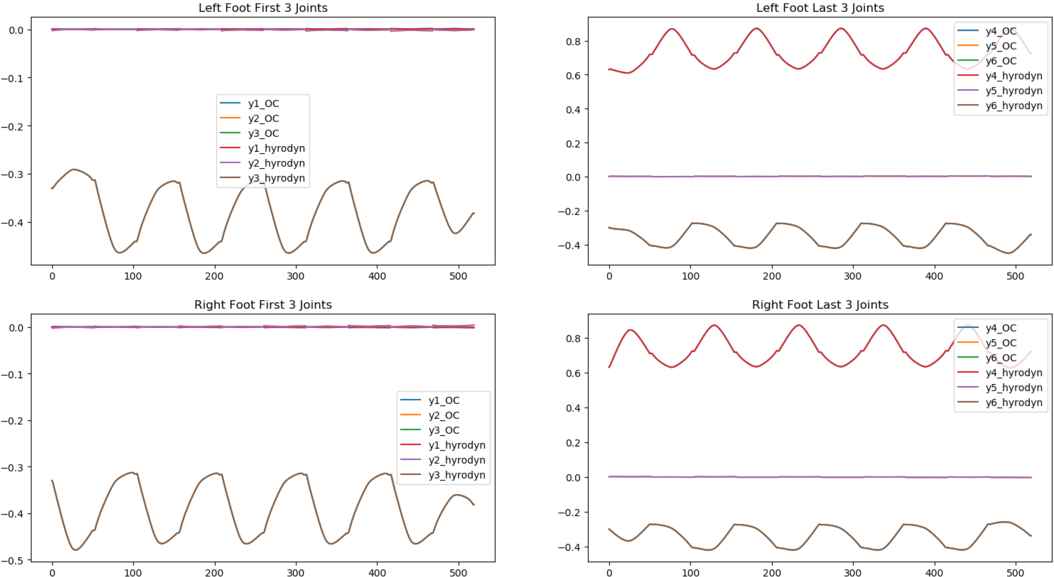
\includegraphics[width=1\textwidth]{fig/hyrodyn/ik_comparison}
\caption[Inverse Kinematics Consistency Check.]{Inverse Kinematics Consistency Check.}
\label{fig:frameworkConsistency_ik}
\end{figure}

\subsection{Inverse Dynamics}
\begin{figure}[h!]
\centering	
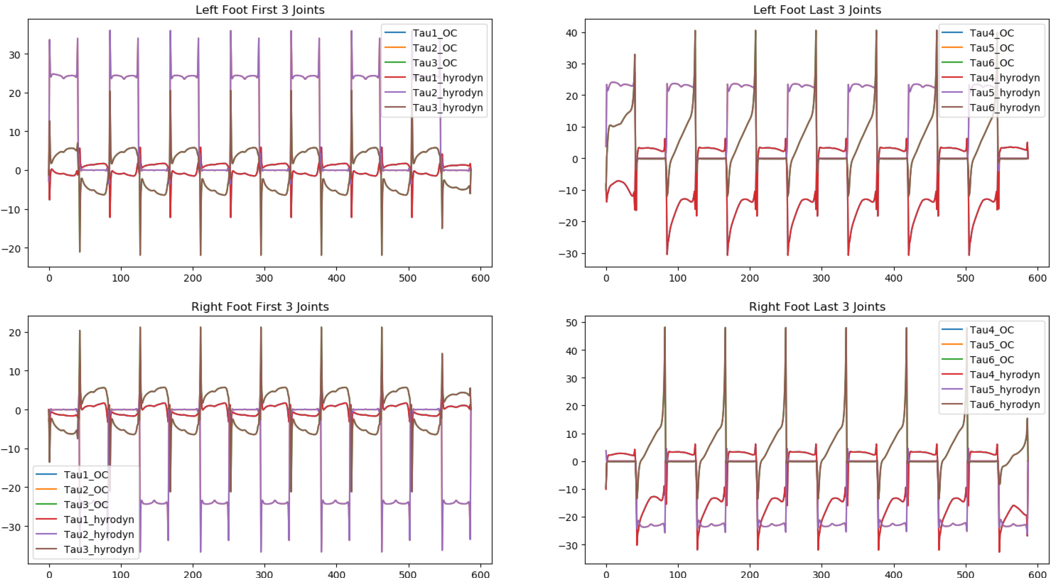
\includegraphics[width=1\textwidth]{fig/hyrodyn/id_comparison}
\caption[Inverse Dynamics Consistency Check.]{Inverse Dynamics Consistency Check.}
\label{fig:frameworkConsistency_id}
\end{figure}















